\section{Sistema Nervioso}

%\textbf{¿Qué es una neurona?} 
%Las neuronas son cuerpos con dendritas que tienen %unos núcleos que transfieren electricidad, que %tienen un axón y la electricidad viaja del cuerpo %de la neurona a través del axón y estas se conectan %entre sí.

\textbf{¿Qué es un nervio?}
Un nervio es una gran colección de axones que están viajando todos juntos como en una especie de cable (poner el corte), pasan vasos sanguíneos por en medio de los nervios, esto es de lo que está formando el sistema nervioso, que cubre desde el cerebro, la médula espinal y todos aquellos elementos que salen de ahí.

Los nervios son estructuras conductoras de impulsos nerviosos situados fuera del sistema nervioso central, es decir, estamos hablando de todos estos axones que salen desde del cráneo, la médula espinal y están descubriendo el resto del cuerpo.
Están formados por un conjunto de axones agrupados cada uno de los cuales procede de una neurona. Pueden ser clasificados como:

\begin{itemize}
\item \textbf{Motores} salidas, ejecución/acción  
\item \textbf{Sensitivos} entradas 
\item \textbf{Mixtos} son mayoría, tienen tanto fibras sensitivas como motoras
\end{itemize}


Tenemos dos grandes partes del sistema nervioso, el \textbf{sistema nervioso periférico} y el \textbf{sistema nervioso central}, como se puede ver en la imagen \ref{fig:SNCySNP}. 

%(Insertar esquema) 
\begin{figure}[h]
 \centering
 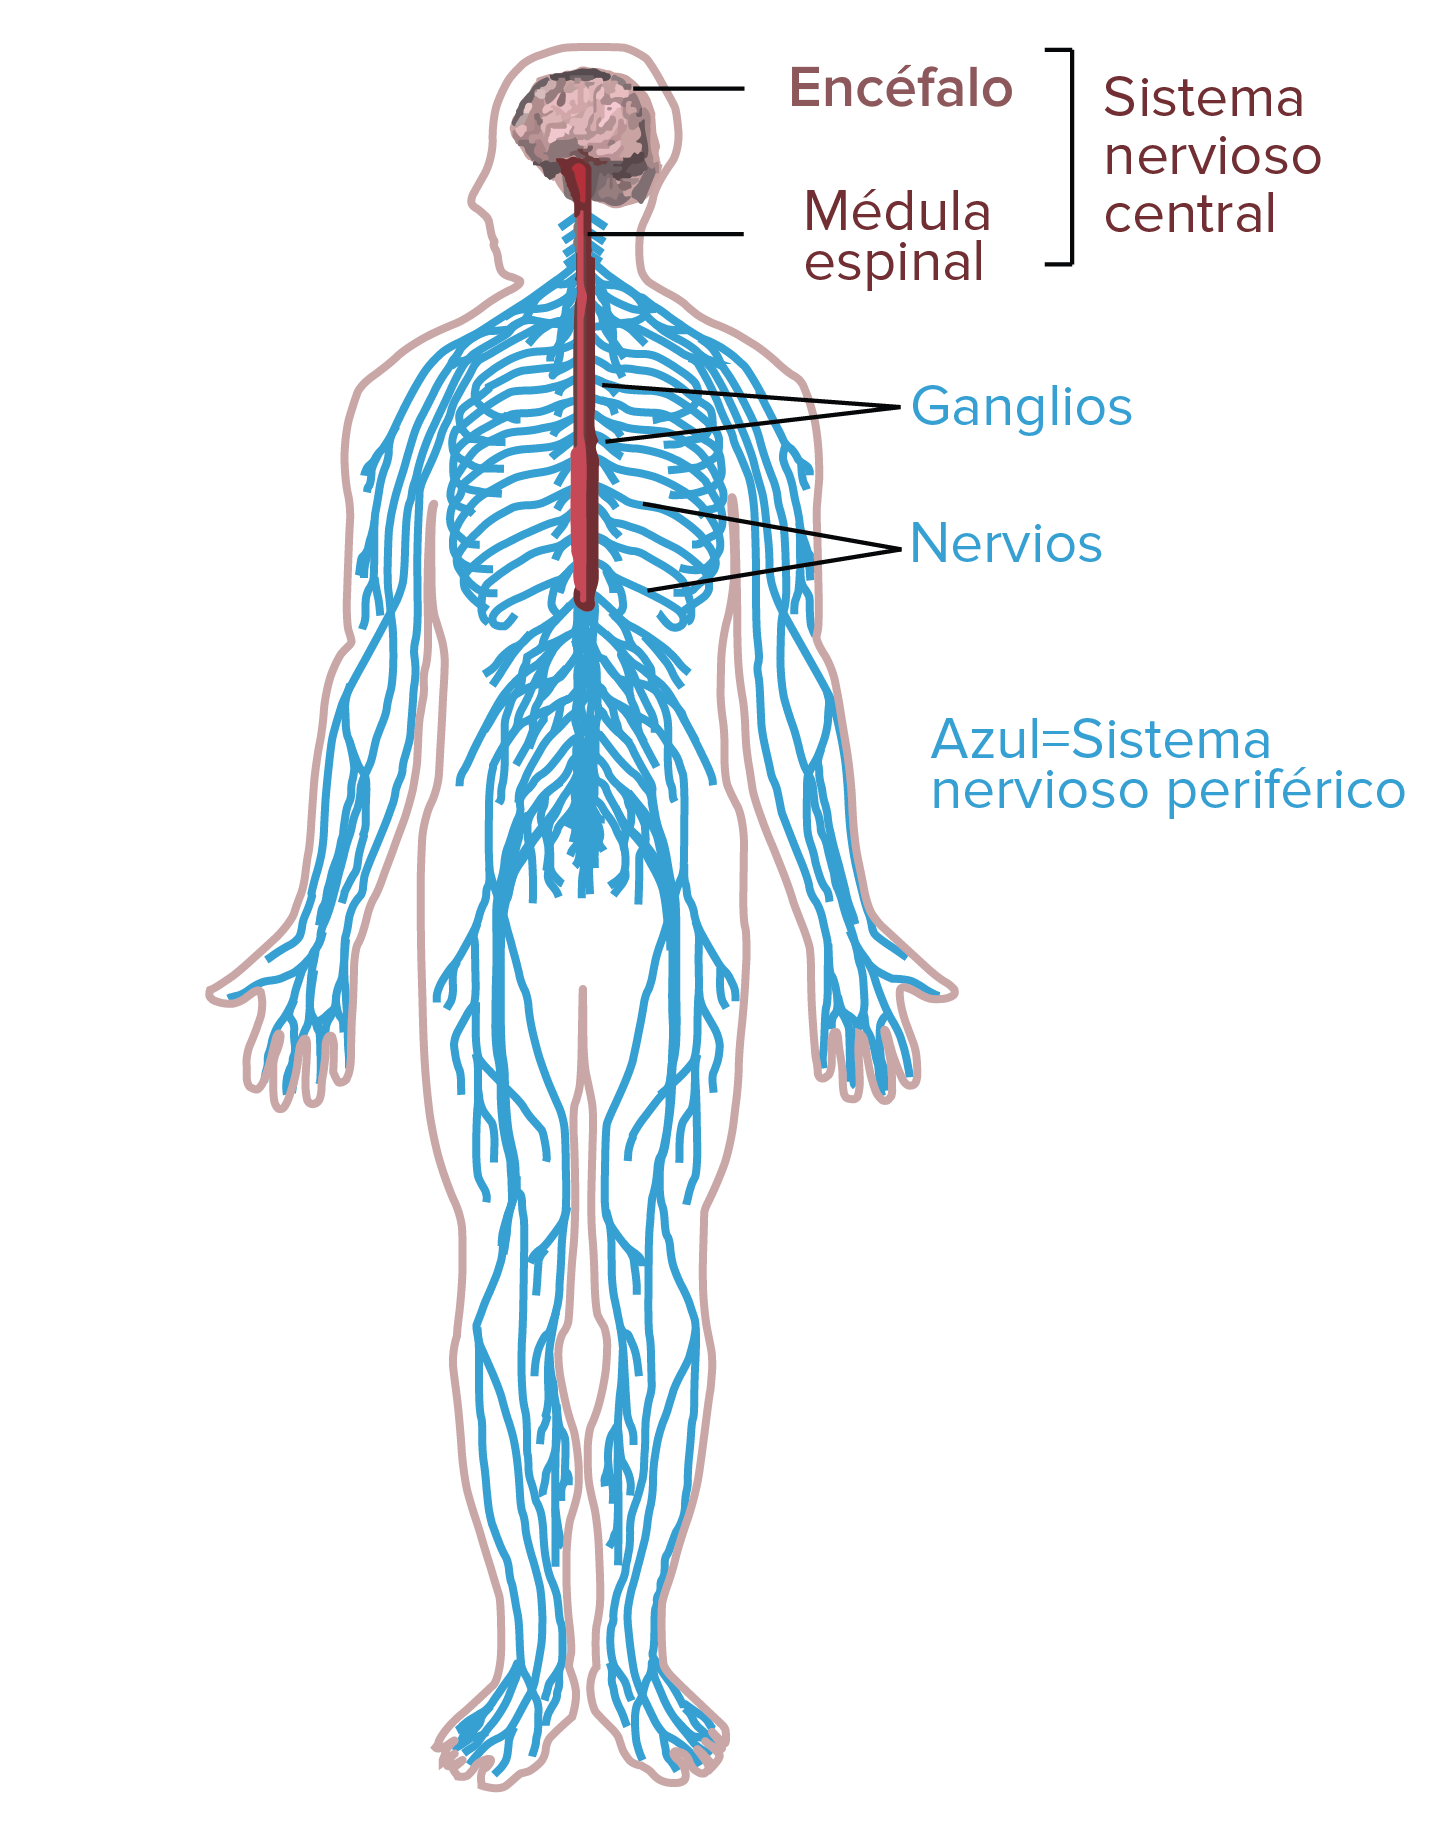
\includegraphics[scale=0.5]{../Figuras/SNCySNP.png}
%  %https://cdn.kastatic.org/ka-perseus-images/9a9a426018284bb704f997cb21944de7ca669e12.png
  \caption{En rojo el sistema nervioso central y en azul el sistema nervioso periférico.}
  \label{fig:SNCySNP}
\end{figure}

En del sistema nervioso periférico tenemos al:

\begin{itemize}
 \item \textbf{Sistema somático} se controla de forma voluntaria, se conforma de nervios conectados a músculos voluntarios esqueléticos y receptores sensoriales, de los cuales unos son:
 \begin{itemize}
  \item de entrada, \textbf{aferentes}
  \item de salida, \textbf{eferentes}
 \end{itemize}
\begin{figure}
 \centering
 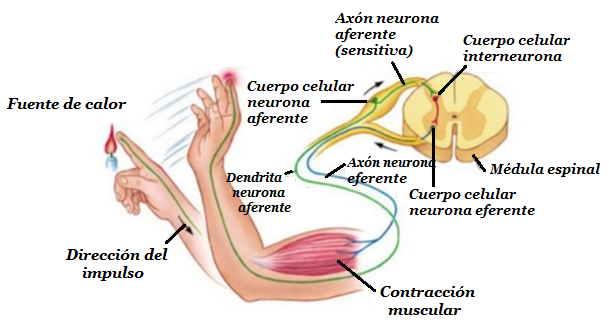
\includegraphics[scale=0.7]{../Figuras/actoreflejo2.png}
%  %http://biologiapuntocom.blogspot.com/2013/06/arco-reflejo.html
  \caption{Vemos como el receptor sensorial aferente, notifica de una fuente de calor muy cerca del nervio y el receptor sensorial eferente manda una respuesta motora.}
  \label{actReflejo}
\end{figure}
 
\item \textbf{Sistema autónomo} funciona de forma involuntaria, se conforma de nervios que se conectan con el corazón, los vasos sanguíneos, los pulmones, el estómago, los intestinos, glándulas
\end{itemize}

Ahora respecto al sistema nervioso central lo integra:

\begin{itemize}
 \item La médula espinal
    \begin{itemize}
     \item Dentro de esta hay una organización, la presencia de \textbf{ciclos de retroalimentación local}, es decir, nuestro sistema va a estar en diferentes etapas son nervios que no necesitan pasar por todo el procesamiento cerebral, las señales simplemente entran llegan a una fase local e inmediatamente reaccionan, ver el ejemplo de la imagen \ref{actReflejo}. Ocurren en un ciclo local y esto también puede convertirse en algo muy importante a la hora de hacer cómputos, no siempre es necesario pasar todo por todas las capas de procesamiento. 

     \item \textbf{Señales de control motor descendientes} del cerebro hacia las neuronas motoras, estas son señales que provienen de un campo en una capa mucho más alta de procesamiento y provocan movimientos.
     
     \item \textbf{Axones sensoriales ascendentes} donde el cuerpo de la neurona está afuera y la información va a viajar hacia arriba, desde los músculos, piel y  estas señales viajan hasta el cerebro, ver \ref{axonesSA} . 
     \begin{figure}[h]
 	 \centering
 	 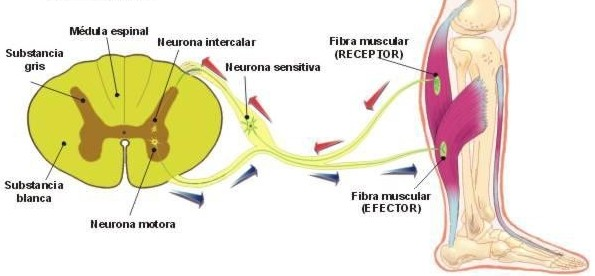
\includegraphics[scale=0.7]{../Figuras/actoreflejo.jpg}
  	 %http://biologiapuntocom.blogspot.com/2013/06/arco-reflejo.html
  	 \caption{La persona ha recibido un estilumo en su musculo posterior de la pierna, provocando un llamado inmediato a sus neuronas sensitivas y generando una respuesta por parte de las neuronas motoras.}
  	 \label{axonesSA}
     \end{figure}
     \end{itemize}

 \item El encéfalo
\end{itemize}

 Cada colección de nervios que sale de la base del cerebro se asocian con funciones muy específicas (en su mayoría). 
 
 Notas:
 
 \begin{itemize}
  \item Este sistema está hecho en diferentes niveles locales, entradas y salidas  
  \item El procesamiento que esté ocurriendo en el encéfalo puede tener diferentes capas y eso se verá reflejado cuando nosotros definamos arquitecturas para las redes neuronales. 
  \item Las redes neuronales actuales, que han tenido más éxito, se componen de diferentes subunidades o diferentes redes que hacen cosas locales. Es decir esta estructura global que estamos viendo,  se está empezando a reproducir/imitar ya con las neuronas computacionales.

 \end{itemize}


\subsection{Cerebro}

En esta parte vamos a preocuparnos sobre todo por la parte funcional. Haciendo una breve analogía, vamos a hacer una visión general del “hardware”, para ver qué efectos va a tener en el “software”. 
En general la arquitectura de cada cerebro es completamente diferente al cerebro de otras personas. Se ha intentado averiguar qué está haciendo cada región con diferentes estudios por ejemplo,  ver cuánta sangre se está bombeando en diferentes regiones del cerebro dependiendo de los estímulos que se le presentan a una persona, o si alguna persona tiene un padecimiento se tratan de tomar escaneos para ver qué regiones del cerebro están funcionando y cuáles presentan lesiones. A partir de las lesiones, lo que hacen es que una vez que está identificada la actividad que ya no se puede realizar de forma normal, averiguan qué región era responsable de esa actividad, que ahora está dañada.

Gracias a esos estudios, se ha logrado identificar más o menos en forma general, a qué se dedica cada una de las regiones del cerebro. En ocasiones no se puede decir exactamente qué tan vinculadas están (las regiones) o por qué se están activando otras regiones.

Hay partes funcionales que se comparten entre las diferentes regiones y no están ubicadas en un solo lugar. Otras parte importante a mencionar es, el cerebelo que se considera prácticamente vital, cumple con funciones tales como el equilibrio, la coordinación, el control fino de los músculos, de hecho tiene más neuronas que el cerebro y aún así hay niños que nacen y viven sin cerebelo. 


A continuación se mencionan algunas de las diferentes funciones de las regiones, que se han identificado en la imagen \ref{cerebro}: 

 \begin{figure}[h]
  \centering
  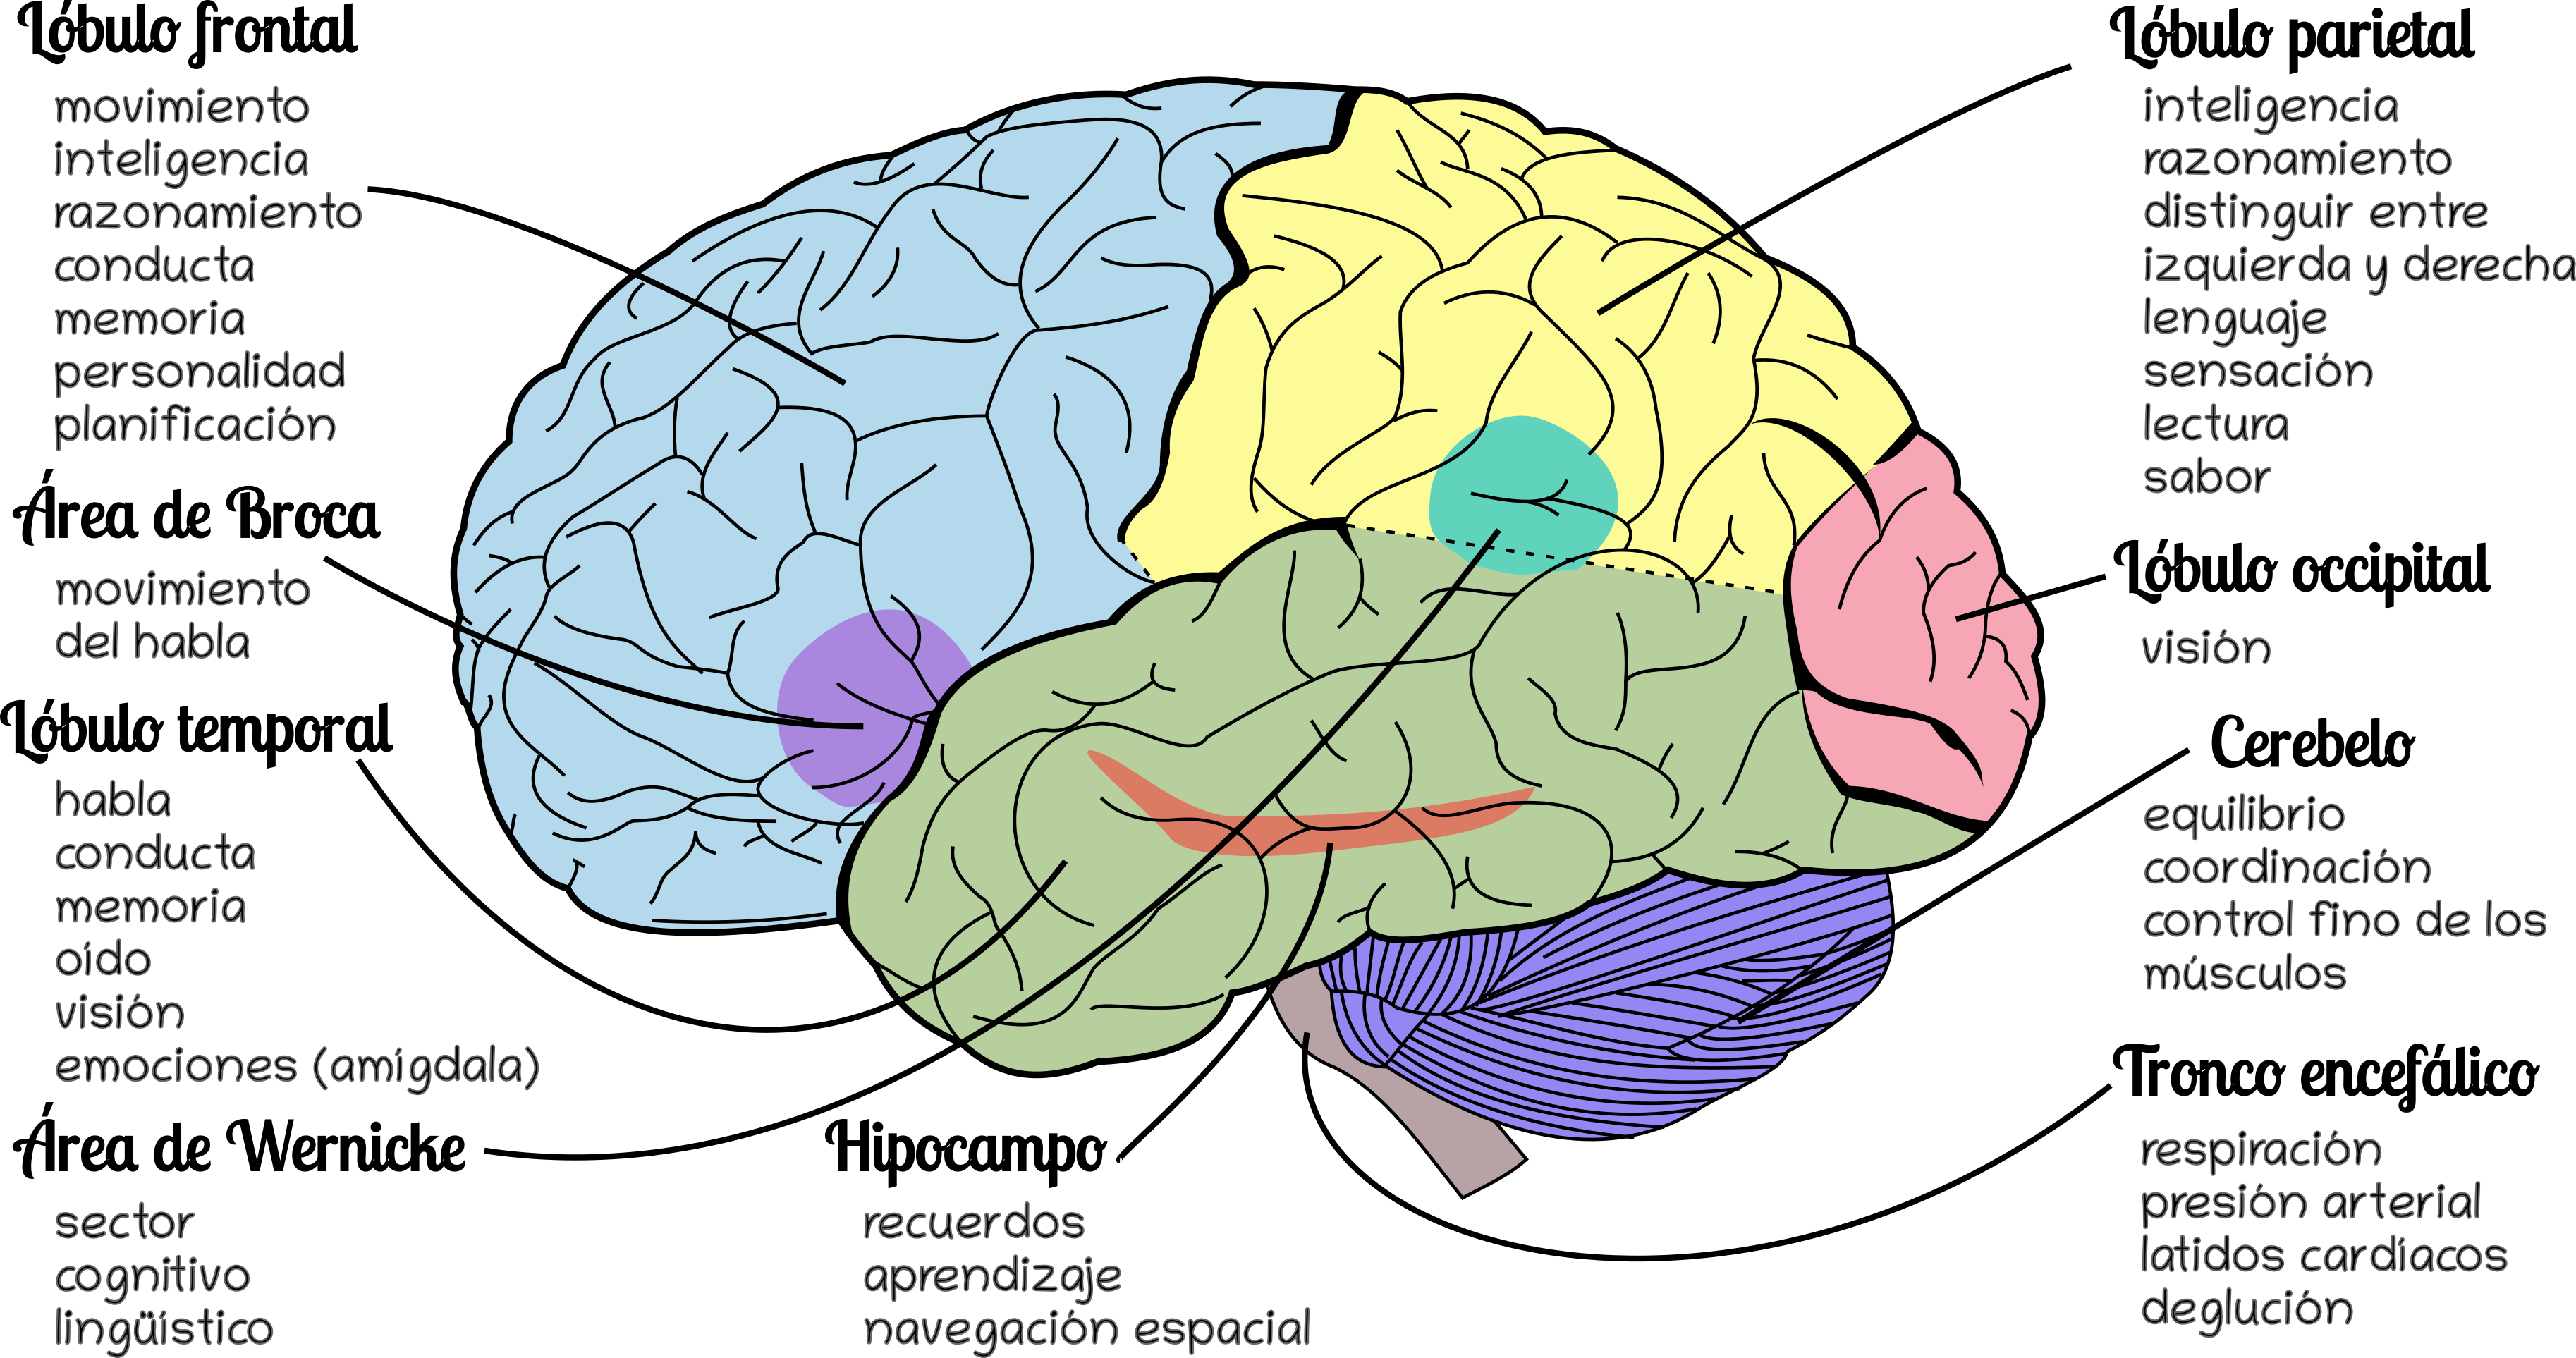
\includegraphics[scale=0.7]{../Figuras/cerebro.png}
  %Presentación Sistema Nervioso
  \caption{Diagrama básico de las regiones del cerebro.}\label{cerebro}
 \end{figure}

\begin{description}
%\begin{itemize}
 \item \textbf{Lóbulo frontal} se le puede asociar con la parte del raciocinio,  la parte de inteligencia, la conducta, la memoria, la personalidad, la capacidad para realizar planes complejos a largo plazo y también es responsable de algunas actividades de movimiento. Dentro de este destaca el área de broca, su principal función es el movimiento del habla, mover los labios, la boca.
 \item \textbf{Lóbulo temporal} aquí está otra parte del habla, que tiene que ver más con el uso de símbolos para el lenguaje, la conducta, memoria, aquí se procesa el oído, un poco de visión y emociones. Dentro de este está (compartida entre el lóbulo parietal) el área de Wernicke, trabaja con la parte lingüística, y de cognición. También dentro de este está el \textbf{hipocampo} trabaja con recuerdos, aprendizaje y navegación espacial, cómo sabemos cómo llegar de un lado hacia otro.
 \item \textbf{Lóbulo parietal} trabaja con la inteligencia, razonamiento, distinguir entre izquierda y derecha, lenguaje, sensación, lectura y sabor. 
 \item \textbf{Lóbulo occipital} se dedica prácticamente solamente a visión, es una región un tanto amplia. En particular en el área de robótica cuando están programando un robot o móvil, los robots tienen dos laptops y una de ellas se dedica prácticamente solo a procesar la visión.
 \item \textbf{Cerebelo} se encarga del equilibrio, la coordinación fina de los músculos.
 \item \textbf{Tronco encefálico} se encarga de la respiración, presión arterial, latidos cardíacos, de ilusión, conciencia. 
%\end{itemize}
\end{description}

\subsection{Zonas funcionales}
Para visualizar mejor la parte de la arquitectura, que tiene el cerebro para realizar todo lo que se le conoce como,  la ruta desde la sensación hasta la cognición, veremos un diagrama de la parte funcional del cerebro.  

 \begin{figure}[h]
  \centering
  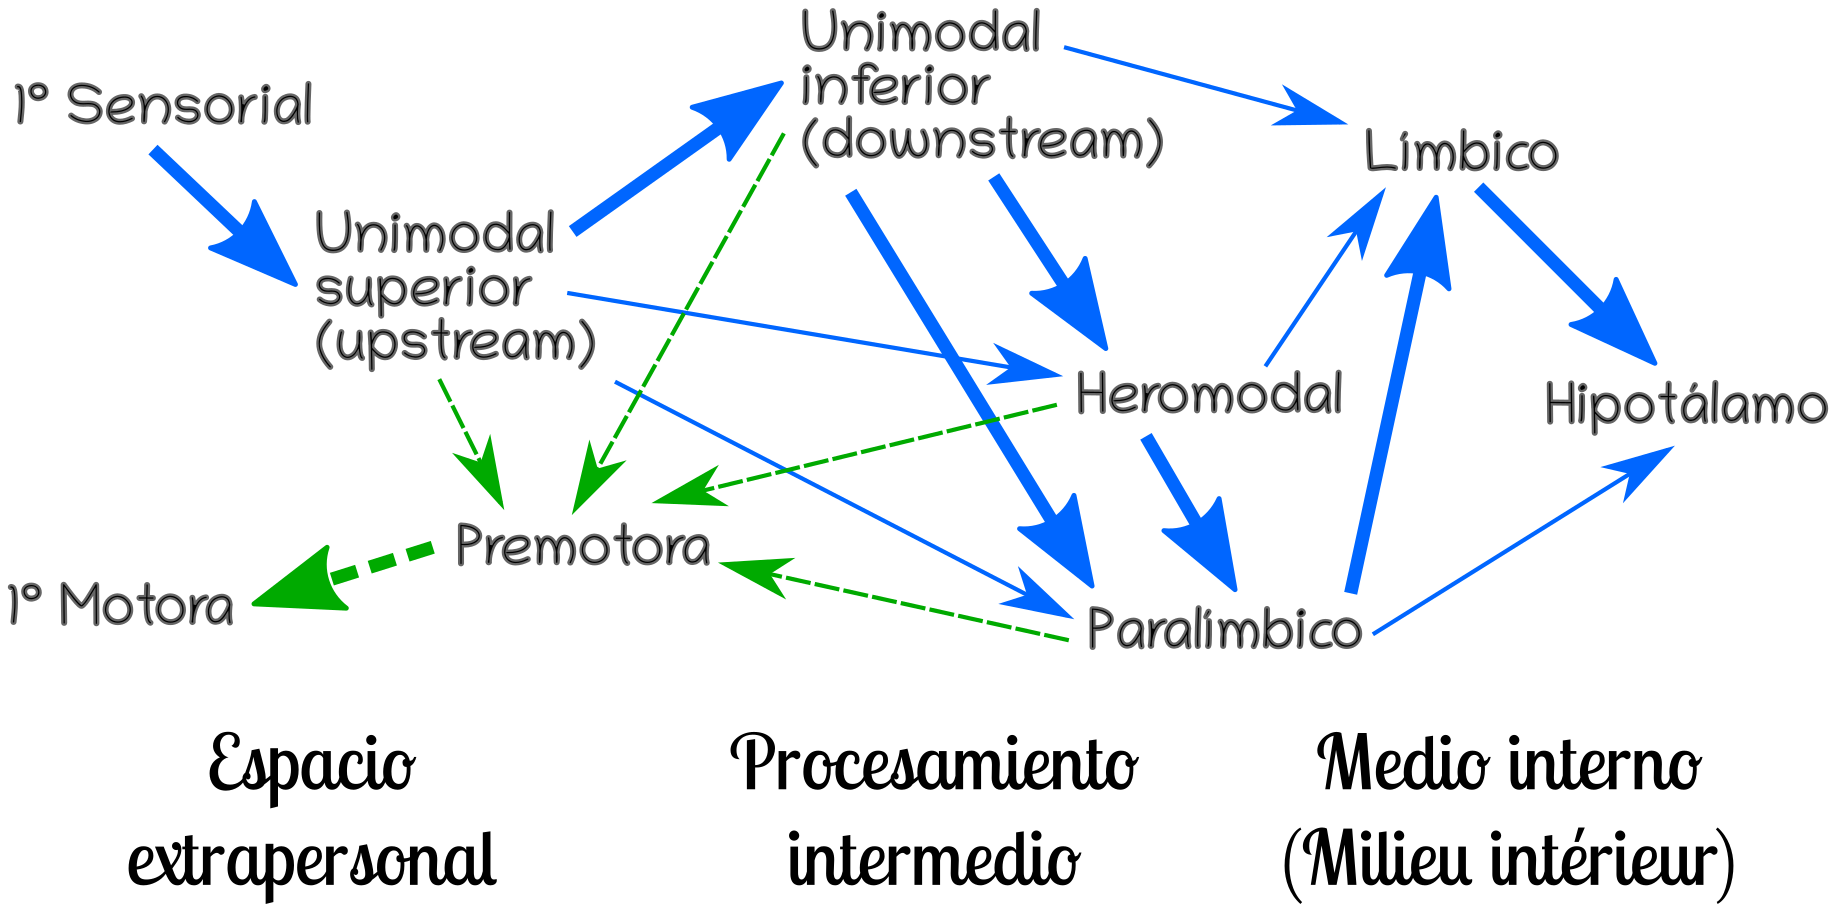
\includegraphics[scale=0.2]{../Figuras/zonasFuncionales.png}
  %Presentación Sistema Nervioso (11)
  \caption{Diagrama de la arquitectura del cerebro a nivel funcional.}
  \label{zonasFun}
 \end{figure}

Explicando el diagrama \ref{zonasFun}, en la primera parte (espacio extrapersonal) vamos a pensar en la entrada sensorial, que se enfoca muchísimo en la parte de visión y audio (en general todos los sentidos), notamos qué de las neuronas que están en la parte sensorial, su primera conexión es hacia una capa que se le llama unimodal superior,  aquí se procesa la información de cada sentido de manera individual, es decir, las neuronas o solamente están procesando visión o solamente audio, todavía no se mezclan, por ejemplo de visión, se separan colores e intensidad lumínica, se empieza a detectar algunas esquinas, alguna inclinación, la dirección de las luces y las sombras. Notemos que desde aquí hay una rápida conexión a la sección premotora y luego hacia la parte motora, recordando la mención de los circuitos locales y de reflejos, aquí prácticamente lo podemos ver (en este pequeño camino).

Pasando de este primer procesamiento básico entramos al siguiente que es el unimodal inferior, (aquí aún se está trabajando con procesamiento de una sola modalidad) visión sigue siendo visión, audio sigue siendo audio, pero ya son procesamientos un poco más complejos, por ejemplo, reconocimiento de rostros, de objetos. En esta parte tenemos un rápido ciclo de regreso a la parte premotora, por ejemplo la acción de ver a mi mamá y saludarla (aquí aún no se tiene que razonar demasiado). 

En la siguiente fase (medio interno), se conecta hacia tres áreas, la \textbf{heromodal}, ya se integran diferentes modalidades (audio y visión) ejemplo, oigo que me hablan y volteo a ver, aquí se está juntando ambas cosas, el \textbf{límbico} y el \textbf{paralímbico} que trabajan con la parte de las emociones y conceptos abstractos.

Finalmente llegamos al \textbf{hipotálamo} que es donde están todas las emociones, en las conexiones entre estas regiones, estarían los procesamientos de alto nivel.

Ahora estas diferentes regiones se replican de cierta manera cuando estamos haciendo los diseños de las arquitecturas modernas para redes neuronales.
En algunas ocasiones se comienza con algunas capas de neuronas, haciendo procesamientos con una sola modalidad, extrayendo datos básicos, después se van
componiendo en figuras más complejas y después hasta podemos combinar bloques de neuronas, para poder resolver problemas que tomen en cuenta diferentes modelos.



